\documentclass[10pt,twocolumn,letterpaper]{article}

\usepackage{cvpr}
\usepackage{times}
\usepackage{epsfig}
\usepackage{graphicx}
\usepackage{amsmath}
\usepackage{amssymb}
\usepackage{listings}

% Include other packages here, before hyperref.

% If you comment hyperref and then uncomment it, you should delete
% egpaper.aux before re-running latex.  (Or just hit 'q' on the first latex
% run, let it finish, and you should be clear).
\usepackage[breaklinks=true,bookmarks=false]{hyperref}

\graphicspath{ {images/} }

\cvprfinalcopy % *** Uncomment this line for the final submission

\def\cvprPaperID{****} % *** Enter the CVPR Paper ID here
\def\httilde{\mbox{\tt\raisebox{-.5ex}{\symbol{126}}}}

% Pages are numbered in submission mode, and unnumbered in camera-ready
%\ifcvprfinal\pagestyle{empty}\fi
\setcounter{page}{1}
\begin{document}

%%%%%%%%% TITLE
\title{Comparing Attention Mechanisms on Car-Racing Variants}

\author{Amrith Arunachalam\\
    Columbia University\\
    IEOR 4540\\
    {\tt\small aa4053@columbia.edu}
    % For a paper whose authors are all at the same institution,
    % omit the following lines up until the closing ``}''.
    % Additional authors and addresses can be added with ``\and'',
    % just like the second author.
    % To save space, use either the email address or home page, not both
}
\maketitle
%\thispagestyle{empty}

%%%%%%%%% ABSTRACT
\begin{abstract}
    Implicit and Explicit Attention have in previous works shown to 
    have trade-offs between performance and generalizability. Through this
    report we propose a new method of attention that draws from both implicit
    attention and explicit attention to leverage the benefits of both. 
    We test these results on the Car-Racing Simulation Environment and 
    its variants. We demonstate that the theoretical performance gain exists in 
    our empirical testing.
  
\end{abstract}

%%%%%%%%% BODY TEXT
\section{Introduction}

The Transformer Architecture was devised to help in the language processing space
but has since seen application to various other domains including vision-based learning problems. 
For our uses, we will be looking at the attention mechanism originally proposed by \cite{Vaswani}. 
More specifically, we will be comparing the explicit attention bottleneck approach taken 
by \cite{Tang} with the implicit attention for pixels algorithms proposed by \cite{choromanski}.

\begin{figure}[h]
    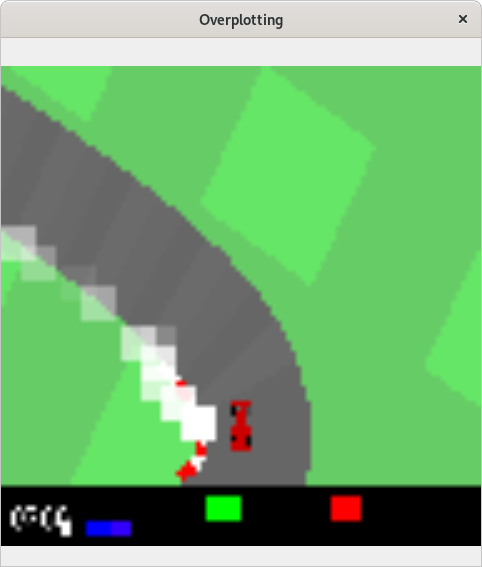
\includegraphics[scale=0.24]{images/intro1.png}
    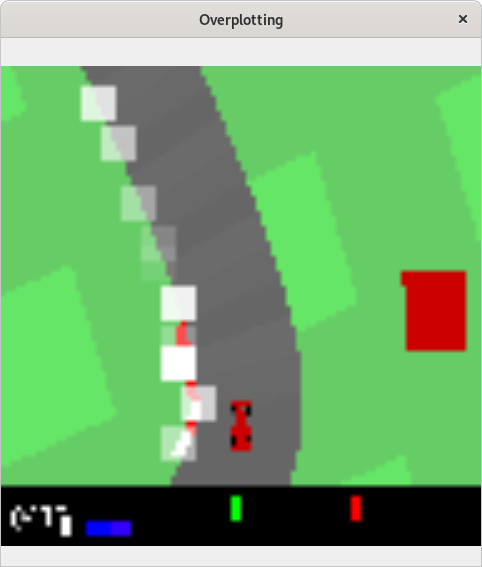
\includegraphics[scale=0.24]{images/intro2.png}
    \caption{Car-Racing simulation and its variants}
    \label{fig:intro}
\end{figure}

\subsection{Self-Attention Bottleneck}
The purpose of the attention mechanism is to learn how the input interacts with itself(through
ES techniques)
and help the controller weigh the more important areas using an importance matrix.
The controller learns which of the inputs to pay more "attention" to and follows the 
neurovolution seen in humans. The output of the attention layer 
is the importance or attention to be placed on a given pixel/patch in a image. The output
is sent to a controller module that controls our agent's actions. The use of an 
attention layer 
inroduces a performance bottleneck for the Transformer architecture. Self-attention as 
calculated in \cite{Tang} is as follows:
$$ A = softmax(\frac{1}{\sqrt{d_{in}}} (XW_k)(XW_q)^\top) $$
We note that in the process of calculating this attention matrix we take a softmax of a matrix size 
$A   \epsilon  R^{n x n}$ in addition to manually computing and storing the complete 
matrix. This encourages practitioners to reduce the size of the attention matrix as much 
as possible. While there are some benefits to using a smaller attention matrix (better generalization),
there are certainly cases where being able to use smaller patches and even using pixels in the Attention
matrix would be useful.

\subsection{Implicit Attention For Pixels}
The work performed initally by \cite{Performers} showed a new technique for performing attention and 
generalized the concept such that they introduced kernel transformations. This meant we could approximate 
the softmax used by \cite{Tang} with the performance gains of using the FAVOR+ algorithm. This next step is 
shown in the development of the IAP-Rank algorithm which uses the attention bottlenecks found in \cite{Tang}
in combination with the FAVOR+ algorithm to produce faster training and equal if not better performance in tests. \\
As compared to the method used by \cite{Tang}, the attention matrix calculated via 
FAVOR+ goes as folllows:\\
$$\hat{Att}(V) = \Xi ((P_{1,L}Q')(K')^\intercal,V)$$
Instead of calculating the Attention matrix outright, by disentangling $Q'$ from $K'$ we 
compute the input in linear(as compared to quadratic) time and space. In this report we
not only compare explicit attention and implicit attention but we also compare two 
kernels used with IAP-Rank ($softmax$ and $ReLU$).

In this report, we focus on comparing IAP-Rank with 
\cite{Tang} as we feel that this comparison is the most natural and will lead to 
interesting discussion.

\begin{figure}[h]
    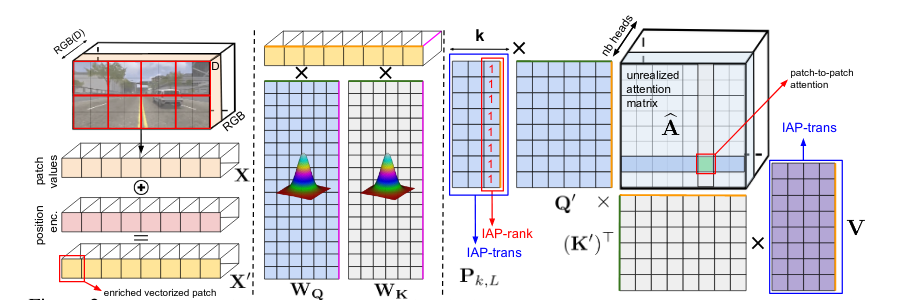
\includegraphics[scale=0.26]{images/iap.png}
    \caption{IAP Architecture \cite{choromanski}}
\end{figure}


%------------------------------------------------------------------------
\section{Method}

\subsection{Implementation Details}
Google Brain Tokyo has kindly provided a github repository containing the code 
to reproduce the results they achieved in their paper\cite{Tang}. As a starting
point, we initially trained our model locally to get a
baseline accuracy and model performance. Interestingly, without changing any
hyperparameters and following the same steps as the authors, our model performed
slightly worse. We believe the authors have reduced the 
hyperparameter weights from what they used to train the original models (reduced iterations of ES).
From this starting point, we then found an implementation of Performers 
\cite{Performers} and refactored the code provided by \cite{lucidrains}. Using
the provided FastAttention class as a base, we were able to implement
IAP-Rank as detailed in \cite{choromanski}. To test the different kernel implementations
we changed the attn\_fn variable to reflect the appropriate kernel.

\subsection{Controller}
\begin{table}[h]
\centering
\caption{\label{tab:config}Config Variables}
\begin{tabular}{|l|l|}
\hline
Variable                                              & Values \\ \hline
VisionTaskSolution.patch\_size & [1,3,5,7]    \\ \hline
VisionTaskSolution.patch\_stride & 4   \\ \hline
utility.create\_task.modification          & ['original','color',   \\ 
                                            & 'bar','blob']   \\ \hline
\end{tabular}
\end{table}
We take the output from our attention mechanism and use it to train our controller that
determines the movement of the car. For consistency across different experiments, we 
used the same controller architecture as suggested by \cite{Tang} with modifications to
the input shape to the LSTM layer and the multi-layer perception class.
These modifications allow us to experiment with various patch sizes from as granular 
as a pixel to as general as the whole image.
For our different experiments we adjusted the variables found here \ref{tab:config}

\begin{figure}[h]
    \includegraphics[scale=0.29]{images/Tang.png}
    \caption{Attention Bottleneck Architecture \cite{Tang}}
    \label{fig:tang}
\end{figure}

\subsection{Training Environment}
All tests conducted were performed in a GNU/Linux(Debian) VM running on a Windows laptop 
with an Intel 6-core CPU.
This introduces bias in our results as the experiments were not
conducted under replicable conditions.\\
To reproduce the environment please use python 3.9.2 and activate a virtual environment
of your choice. From here download the necessary libraries using the following command 
from the project root directory:
\begin{lstlisting}[language=bash]
  $ pip install -r requirements.txt
\end{lstlisting}

%------------------------------------------------------------------------
\section{Results and Discussion}

In this section we compare the performance of explicit attention mechanisms with 
implicit attention mechanisms from training performance, training scores
and testing scores.

\subsection{Training Agents}

\begin{figure}[h]
    \caption{Training Times For Various Experiments}
    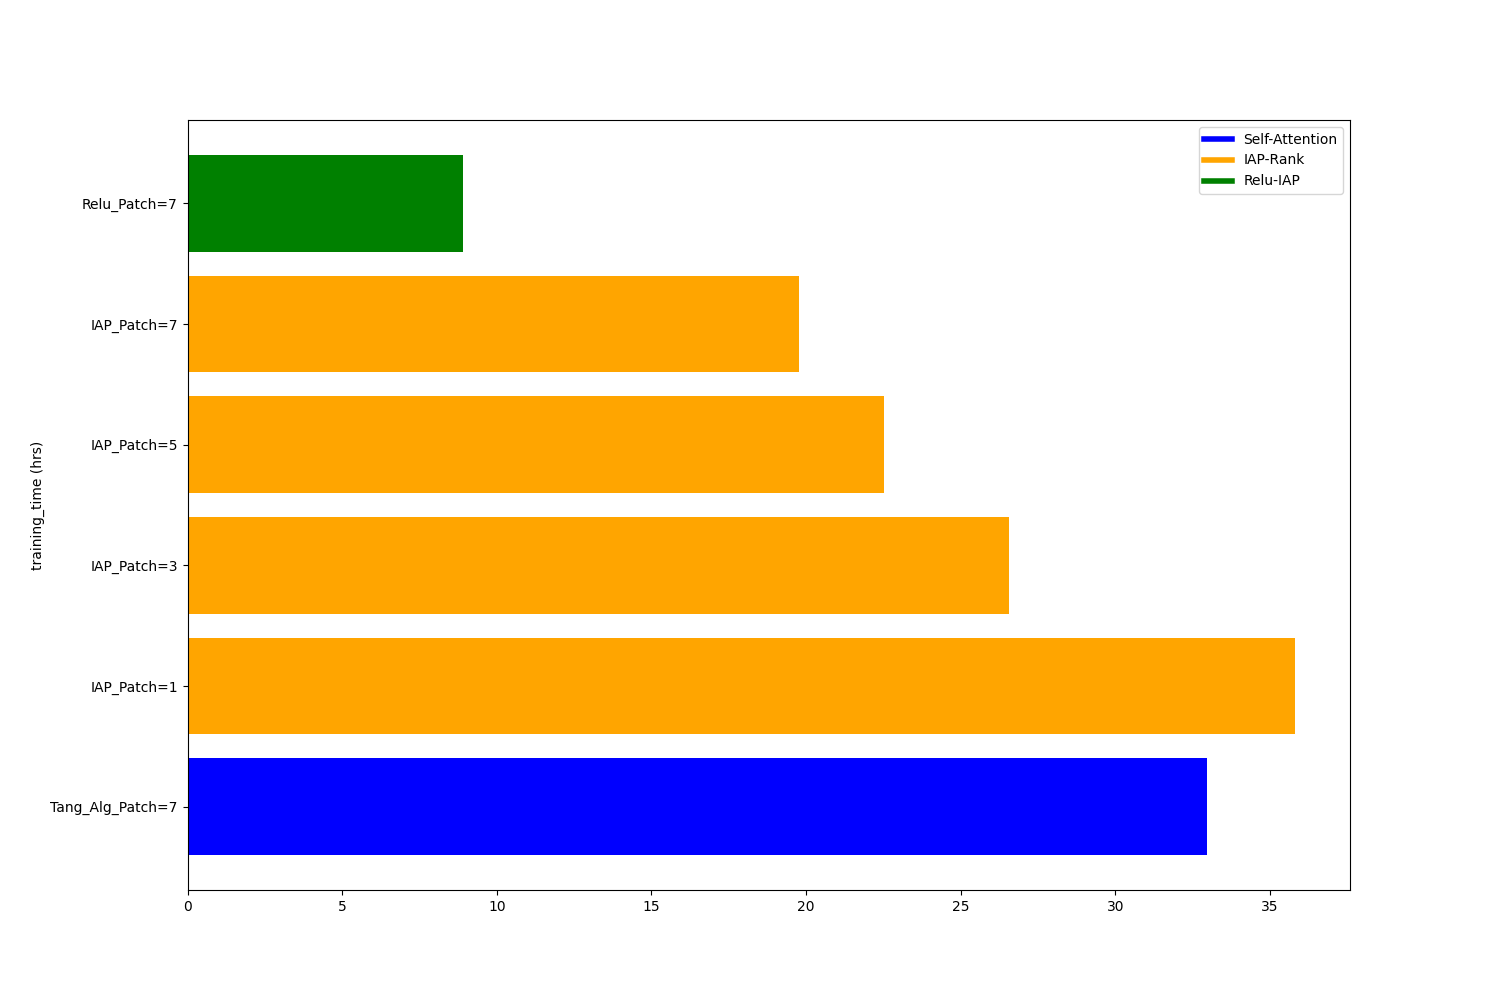
\includegraphics[width=83mm, scale=0.9]{images/training_plot.png}
    \label{fig:train}
\end{figure}

In this section we will discuss the training times for various attention mechanisms.
Our testing methodology is as follows, we used the same Transformer RL model for all
models only replacing the attention mechanism for the 3 varieties. We started by 
using the Self-Attention Bottleneck described by \cite{Tang} which took the second 
most amount of time. We then used our implementation of IAP-Rank with the softmax kernel
approximation and 25 random orthogonal projections. 
See \ref{fig:train} for specifics regarding each individual trial, overall we see that 
as expected the training time decreases as we increase patch size, this makes intuitive 
sense as the attention matrix decreases quadratically by $k^2$ as we increase patch size
by $k$. Finally, as a novel new concept trial, we used the FastAttention layer's 
ability to use different kernels to test using a ReLU kernel approximation and found
that the model had very strong training performance but suffered significantly in the 
test results.

\subsection{Testing Agents}

In this section, we discuss the results achieved by various agents on OpenAI Gym Car-Racing
and it's variants. There are 3 major variants, Self-Attention bottleneck as provided by
\cite{Tang}, IAP-Rank Softmax by \cite{choromanski} and IAP-Rank ReLU by \cite{choromanski}.
Each model is trained on the original track and tested on variations of the original track
10 times. We record the mean and the variance for every model tested. In the root 
directory for this project there is a folder called videos that has videos of trained 
agents performing the vision task. Because we are testing IAP-Rank, we kept the 10 
most important patches as described in the paper.

\begin{table}[h]
\centering
\caption{\label{tab:original}Test Scores on Original Track}
\begin{tabular}{|l|l|}
\hline
model               & score \\ \hline
Original Tang       & $914 \pm 15$  \\ \hline
IAP Softmax Patch=1 & $803 \pm 210$  \\ \hline
IAP Softmax Patch=5 & $751 \pm 51$  \\ \hline
IAP Softmax Patch=7 & $723 \pm 32$   \\ \hline
Tang Patch=7        & $712 \pm 53$   \\ \hline
IAP Softmax Patch=3 & $703 \pm 91$  \\ \hline
IAP ReLU Patch=7    & $599 \pm 192$  \\ \hline
\end{tabular}
\end{table}

The smaller our patch size the better our model fit the training environment. However, it 
should be noted that there is also increased variability in our model's performance with
decreased patch size. We believe this is because the bottleneck is not being adjusted. 
If we were to test multiple bottleneck sizes, the number of experiments would grow by a 
factorial and we leave adjusting this parameter as an exercise for interested readers to test out.
Because the bottleneck was left at size $l = 10$, we kept the $l$ most important patches 
as determined by our attention mechanism. Intuitively, as the patch size decreases, the 
variability in our model increases as the layers following our attention module will have
less information to work with than if the patch size was strictly larger. If our goal was
to make our model perform optimally in a specific training environment, then removing the attention
bottleneck and providing the following layers with the whole image as the importance
matrix would perform better than using a bottleneck. This however, is not the goal of this task as
we want our agent to be generalizable to variation in environment such as the color, bar or 
blob variation to Car-Racing.

%------------------------------------------------------------------------
\subsection{Car-Racing Variants}

\subsubsection{Color}
We can see from \ref{tab:color} that the results on the color changed variant of the
Car-Racing problem follow the results of the original training environment. This follows 
intuition as we do not expect our model to rely on absolute pixel values for color, but
rather the difference between pixels at the boundaries. This can be most clearly seen 
by looking at \ref{fig:intro}, we can see that while the car is moving forward, we 
see that the attention patches are all along the left side of the road, meaning the car's 
control module is making navigation decisions based on where the left side of the road 
is. This introduces an interesting variable in the environment that may be worth exploring
where the road on the left side goes to the edge of the screen. Additionally,
because all of these models are trained on a counter-clockwise track, the attention module
makes the agents follow the left side of the road for control decisions. We postulate
whether training a model on a counter-clockwise track would make the model have importance
for the right side of the track? And with these attached biases, is there a way for us to 
limit the bias by training on both clockwise and counter-clockwise tracks? We assume that the
model would perform worse in training environments but may generalize better and would
overall be considered a better agent.
\begin{table}
\centering
\caption{\label{tab:color}Test Scores  on Color Track}
\begin{tabular}{|l|l|}
\hline
model               & score \\ \hline
Original Tang       & $866 \pm 115$  \\ \hline
IAP Softmax Patch=1 & $783 \pm 325$  \\ \hline
Tang Patch=7        & $717 \pm 142$   \\ \hline
IAP Softmax Patch=7 & $705 \pm 132$   \\ \hline
IAP Softmax Patch=3 & $703 \pm 191$  \\ \hline
IAP Softmax Patch=5 & $692 \pm 147$  \\ \hline
IAP ReLU Patch=7    & $509 \pm 315$  \\ \hline
\end{tabular}
\end{table}
\subsubsection{Bar}
The bar variation of the Car-Racing problem adds two vertical bars either side of the 
screen, changing the visual experienced our agents. Because all agents use the top $k=10$ 
patches from our attention matrix, we can see that the performance of our models do not 
get significantly affected by this change. We note that the IAP-Rank algorithm with
the same hyperparameters as Tang trains at a significantly faster rate and performs 
the same. In future experimentation, it may be interesting to 
set a time allowance for both models to train in and to see how big the performance gap 
is. Based on results from these experiments, we are led to postulate that IAP-Rank would
be heavily favored.
\begin{table}[h]
\centering
\caption{\label{tab:blob}Test Scores on Bar Track}
\begin{tabular}{|l|l|}
\hline
model               & score \\ \hline
Original Tang       & $898 \pm 53$  \\ \hline
IAP Softmax Patch=1 & $804 \pm 205$  \\ \hline
IAP Softmax Patch=5 & $758 \pm 53$  \\ \hline
IAP Softmax Patch=7 & $720 \pm 37$   \\ \hline
Tang Patch=7        & $708 \pm 43$   \\ \hline
IAP Softmax Patch=3 & $698 \pm 93$  \\ \hline
IAP ReLU Patch=7    & $571 \pm 186$  \\ \hline
\end{tabular}
\end{table}

\subsubsection{Blob}
The Blob variant of the Car-Racing problem has a floating rectangle in the peripheral
vision space seen by our agents. This would have a significant impact on RL agents that
do not utilize an Attention Bottleneck, as those agents would have to process those pixels.
Because both models ignore information outside of the most important patches, we
see that while the performance has decreased, the agent's are still performing well.
Our results fall in line with the performance seen by the initial model used in \cite{Tang}.
\begin{table}[h]
\caption{\label{tab:bar}Test Scores on Blob Track}
\centering
\begin{tabular}{|l|l|}
\hline
model               & score \\ \hline
Original Tang       & $900 \pm 35$  \\ \hline
IAP Softmax Patch=7 & $792 \pm 46$   \\ \hline
Tang Patch=7        & $791 \pm 51$   \\ \hline
IAP Softmax Patch=5 & $749 \pm 49$  \\ \hline
IAP Softmax Patch=1 & $717 \pm 231$  \\ \hline
IAP Softmax Patch=3 & $705 \pm 87$  \\ \hline
IAP ReLU Patch=7    & $503 \pm 201$  \\ \hline
\end{tabular}
\end{table}

%------------------------------------------------------------------------
\section{Conclusion}
In this report we apply the FAVOR+ Algorithm proposed by \cite{Performers} using the 
self-attention bottleneck proposed by \cite{Tang} with IAP-Rank by \cite{choromanski}. 
We see that for Car-Racing the application of a attention bottleneck provides better 
generalization as compared to using smaller patch size. However, when we apply the 
FAVOR+ approximation for softmax kernel, we achieve better results in both training and
testing environments than either paper's results. The ability for the model to be trained
quickly and it's generalizability makes it a strong candidate to be applied to other 
vision tasks like other Atari game simulations.

\section{Acknowledgements}
I would like to thank Prof. Choromanski for teaching this course, it has been a 
great experience and while I have been taking the course online, I have enjoyed 
the material greatly. Additionally, I would like to thank all the contributors who 
worked on making both the brain-tokyo and performer-pytorch repositories. Without their
code to base my work on, this project would not have been possible. Additionally, I 
used the sample template from the 2017 CVPR Proceedings to generate this \LaTeX document.

\section{Reflection}
On a more personal note, through the work conducted on this project, I had the 
chance to read and understand some sophisticated code. I had to understand what 
different modules were trying to achieve  and then change it to suit my needs. As 
someone who is still learning python, it was a challenging but rewarding opportunity to 
learn. This project has been an absolute pleasure to work on
and I hope my passion for the material has shown in my presentation of the work this
semester. This research is amazing and I am excited to see it change the world!
Through working on this project, I have a deeper understanding of the 
optimization problems that need to be solved for RL to be viable and I had the
opportunity to apply one such technique to a new task. As an individual with no
prior background in research I found that reading technical papers was quite challenging 
but a great learning opportunity and I enjoyed my foray into research.

{\small
    \bibliographystyle{ieee}
    \bibliography{egbib}
}

\end{document}
